\documentclass{standalone}
%\usepackage{scrtime} % for \thistime (this package MUST be listed first!)
\usepackage{graphicx}
\usepackage{graphics}
\usepackage{xcolor,colortbl}%for changing cell colour
\usepackage{xspace}
\usepackage{tikz-cd}
\usetikzlibrary{decorations.markings}
\usetikzlibrary{calc, arrows}
\usepackage{color,amsmath,amssymb,amsthm,mathrsfs,amsfonts,dsfont}

\colorlet{darkcol}{black!30!white}
\colorlet{lightcol}{black!10!white}
\definecolor{txtcol}{HTML}{F40000}

\begin{document}
	\centering{
	\resizebox{\textwidth}{!}{%
		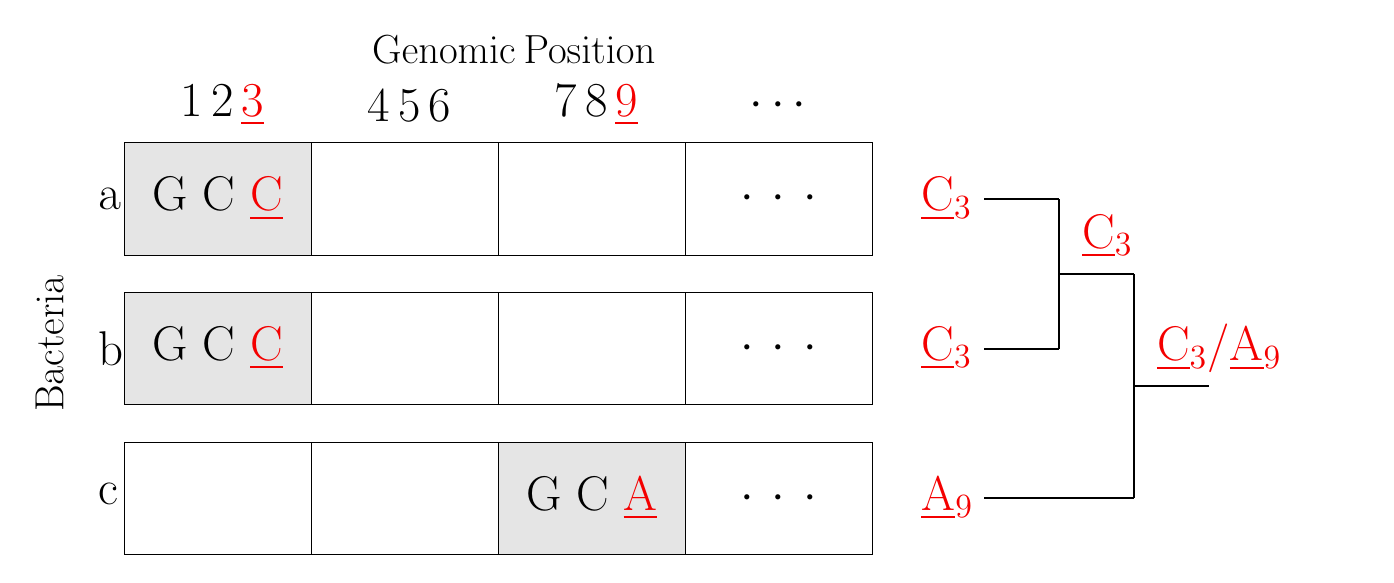
\begin{tikzpicture}[scale = 0.95, every node/.style={scale=0.85}]
	%%%% Genome Pos lable
	\node[text width=6cm] at (6,4.75) {\LARGE Genomic Position};
	\node[text width=3cm] at (2.1,4) {\huge 1 2 \textcolor{txtcol}{\underline{3}}};
	\node[text width=3cm] at (4.6,4) {\huge 4 5 6};
	\node[text width=3cm] at (7.1,4) {\huge 7 8 \textcolor{txtcol}{\underline{9}}};
	\node[text width=3cm] at (9.6,4) {\huge \textbf{ $\cdot$ $\cdot$ $\cdot$}};
	%%%% Bac lable
	\node[text width=3cm, rotate=90] at (-1,1.25) {\LARGE Bacteria};
	\node[text width=3cm] at (1,2.75) {\huge a};
	\node[text width=3cm] at (1,0.75) {\huge b};
	\node[text width=3cm] at (1,-1.2) {\huge c};
	
	%\draw[step=1cm,gray,very thin] (-2,-2) grid (9,4);
	%%%top  bac %%%%%%%%%%%
	\tikzstyle{neleven}=[draw = none, minimum width=2cm, minimum height=0.5cm, rounded corners]
	%		\node[neleven, align=center] (elevenres) at (-1,2) {a}
	%			\draw[color=white] (-1,2) node {a};
	\shade[left color=lightcol,right color=lightcol, draw=black] (0,2) rectangle (2.5,3.5) node[pos=0.5] {\huge G C \textcolor{txtcol}{\underline{C}}};
	\shade[left color=white,right color=white, draw=black] (2.5,2) rectangle (5,3.5);
	\shade[left color=white,right color=white, draw=black] (5,2) rectangle (7.5,3.5);%third block
	\shade[left color=white,right color=white, draw=black] (7.5,2) rectangle (10,3.5) node[pos=0.5] {\huge \textbf{$\cdot$ $\cdot$ $\cdot$}};%fourth block
	%%%%% middle bac %%%%%%%%%
	\shade[left color=lightcol,right color=lightcol, draw=black] (0,1.5) rectangle (2.5,0) node[pos=0.5] {\huge G C \textcolor{txtcol}{\underline{C}}};
	\shade[left color=white,right color=white, draw=black] (2.5,1.5) rectangle (5,0);
	\shade[left color=white,right color=white, draw=black] (5,1.5) rectangle (7.5,0);%third block
	\shade[left color=white,right color=white, draw=black] (7.5,1.5) rectangle (10,0) node[pos=0.5] {\huge \textbf{$\cdot$ $\cdot$ $\cdot$}};%fourth block
	%%%%% bottom bac %%%%%%%%%
	\shade[left color=white,right color=white, draw=black] (0,-0.5) rectangle (2.5,-2);
	\shade[left color=white,right color=white, draw=black] (2.5,-0.5) rectangle (5,-2);
	\shade[left color=lightcol,right color=lightcol, draw=black] (5,-0.5) rectangle (7.5,-2)  node[pos=0.5] {\huge G C \textcolor{txtcol}{\underline{A}}};%third block
	\shade[left color=white,right color=white, draw=black] (7.5,-0.5) rectangle (10,-2) node[pos=0.5] {\huge \textbf{$\cdot$ $\cdot$ $\cdot$}};%fourth block
	
	
	%\shade[left color=eggplant,right color=white, draw=black] (5.5,2) rectangle (7,4);
	
	%%%%%%% Pylo tree %%%
	\draw[thick] (11.5,2.75) -- (12.5,2.75);%bacteria a
	\draw[thick] (11.5,0.75) -- (12.5,0.75);%bacteria b
	\draw[thick] (11.5,-1.25) -- (13.5,-1.25);%bacteria c
	
	\draw[thick] (12.5,2.75) -- (12.5,0.75);%connecting a and b
	\draw[thick] (12.5,1.75) -- (13.5,1.75);%ancest of a and b
	\draw[thick] (13.5,1.75) -- (13.5,-1.25);%connecting ancest and c
	\draw[thick] (13.5,0.25) -- (14.5,0.25);%root
	
	%%%%%%%%%% tree words %%%%
	%%% tips %%
	\node[text width=3cm] at (12,2.75) {\huge \textcolor{txtcol}{\underline{C}\textsubscript{3}}};
	\node[text width=3cm] at (12,0.75) {\huge \textcolor{txtcol}{\underline{C}\textsubscript{3}}};
	\node[text width=3cm] at (12,-1.25) {\huge \textcolor{txtcol}{\underline{A}\textsubscript{9}}};
	%%% nodes %%
	\node[text width=3cm] at (14.15,2.25) {\huge \textcolor{txtcol}{\underline{C}\textsubscript{3}}};
	\node[text width=3cm] at (15.15,0.75) {\huge \textcolor{txtcol}{\underline{C}\textsubscript{3}/\underline{A}\textsubscript{9}}};
	
	%\draw[thick] (7,3) -- (8,3);%last block to right
	%			\draw[thick] (1.5,3) -- (2,3);%first block to second
	%			\draw[thick] (5,3) -- (8,3);%second block to third
	%first block lines across
	%			\draw[thick] (0,2) -- (5.5,0);
	%			\draw[thick] (1.5,2) -- (7,0);
	%second block lines top to bottom
	%			\draw[thick] (2,2) -- (2,0);
	%			\draw[thick] (5,0) -- (5,2);
	%third block lines top to bottom
	%\draw[thick] (5.5,2) -- (0,0);
	%\draw[thick] (7,2) -- (1.5,0);
	
	%%%%bottom row
	%\shade[left color=eggplant,right color=white, draw=black] (0,0) rectangle (1.5,-2);%first block
	%			\shade[left color=teal!55,right color=white, draw=black] (2,0) rectangle (5,-2);%second block
	%			\shade[left color=atomictangerine,right color=white, draw=black] (5.5,0) rectangle (7,-2);%third block
	%			\draw[thick] (-1,-1) -- (2,-1);%first block to left
	%			\draw[thick] (7,-1) -- (8,-1);%last block to right
	%\draw[thick] (1.5,-1) -- (2,-1);%first block to second
	%			\draw[thick] (5,-1) -- (5.5,-1);%second block to third
	\end{tikzpicture}
	}%resiebox
}

	\end{document}